\section{Latent State $H_t$}
\todo{****  THIS IS DUMP FILE *****}
Describe the process of linking kinematics and video (PCA, CCA, etc.).
If we apply any VLAD or encoding, or batching, describe it here:

\begin{itemize}
\item Encoding - Current Status
\begin{itemize}
\item So I've implemented the following encoding method- Latent Content Descriptors (LCD) + VLAD. However, initial results weren't great and I need to see how it performs on milestones clustering.
\end{itemize}


Vector of Locally Aggregated Descriptors (VLAD) image encoding as proposed by \cite{jegou2010aggregating} is a method a feature encoding and pooling method, similar to Fisher vectors. VLAD encodes a set of local feature descriptors $I=(x_1,\ldots,x_n)$ extracted from an image using a codebook $\mathrm{C} = \{c_1, \ldots, c_m \}$ built using a clustering method such as Gaussian Mixture Models (GMM) or K-means clustering.


VLAD was shown to perform better than Fisher vectors and average pooling for encoding multiple frames~\cite{xu2014discriminative}.

\item Temporal Batching - Current Status
\begin{itemize}
\item While batching is supposed to help in video analysis , I've seen good separation of clusters (PCA on conv features) with just individual frames without clustering... I think I need to look into this more and need to test it out with milestones clustering.
\end{itemize}

\end{itemize}



%%%% TABLE 1
                 & Z             &              &               & k+Z          &              &              \\ \hline
                 & CCA           & GRP          & PCA           & CCA          & GRP          & PCA          \\ \hline \hline
SIFT             &          -     &        -     & -0.113$\pm$0.016 & -            & -            & 0.284$\pm$0.122 \\ \hline
AlexNet conv3    & -0.013$\pm$0.012 & 0.117$\pm$0.035 & 0.200$\pm$0.024  & 0.272$\pm$0.112 & 0.281$\pm$0.119 & 0.267$\pm$0.120 \\ \hline
AlexNet conv4    & -0.025$\pm$0.009 & 0.135$\pm$0.013 & 0.213$\pm$0.007  & 0.294$\pm$0.114 & 0.277$\pm$0.134 & 0.273$\pm$0.102 \\ \hline
AlexNet pool5    & -0.029$\pm$0.023 & 0.129$\pm$0.016 & 0.197$\pm$0.009  & 0.281$\pm$0.134 & 0.258$\pm$0.102 & 0.276$\pm$0.128 \\ \hline
VGG conv5\_3     & -0.012$\pm$0.025 & 0.141$\pm$0.010 & \textbf{0.273$\pm$0.018}  & 0.247$\pm$0.099 & 0.287$\pm$0.138 & 0.325$\pm$0.113 \\ \hline
VGG LCDVLAD     & 0.046$\pm$0.020  & 0.012$\pm$0.002 & 0.068$\pm$0.023  & 0.294$\pm$0.088 & 0.331$\pm$0.088 & 0.224$\pm$0.056 \\ \hline
AlexNet LCD VLAD & 0.068$\pm$0.035  & 0.033$\pm$0.001 & -0.063$\pm$0.053 & 0.285$\pm$0.092 & 0.308$\pm$0.098 & 0.243$\pm$0.102 \\ 



% \begin{figure*}[t!]
%     \centering
%     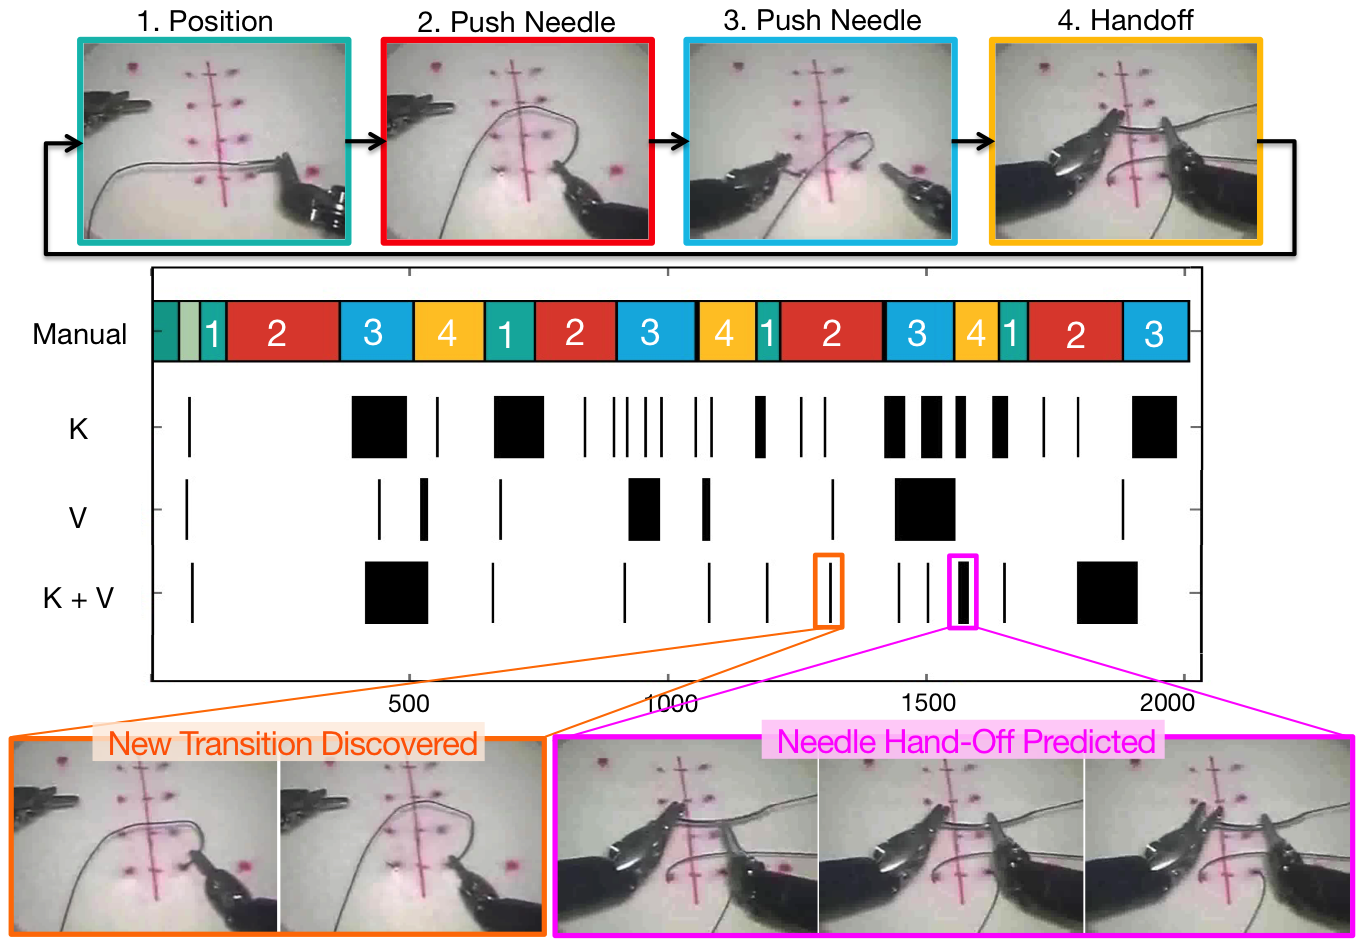
\includegraphics[width=0.8\linewidth]{figures/suturing}
% 	\caption{Suturing: The figure shows a sequence of images for the Suturing in JIGSAWS dataset\cite{gao2014jigsaws}.
% The first row shows a manual segmentation of the task in 4 semantic steps: (1) Needle Positioning, (2) Needle Pushing, (3) Pulling Needle, (4) Hand-off.The task involves 4 repetitions of the 4-step cycle and runs for approx. 100s (frame numbers are at 30 fps). We show the sub-task level segmentation results from our completely unsupervised approach with only Kinematics data, only Visual data and a concatenation of both. The figure also shows (in magenta) frames of predicted Needle Hand-off, and (in orange) a new transition for needle re-orientation between needle push and needle pull.
% }
% 	\label{fig:suturing}
% 	\vspace{-5pt}
% \end{figure*}


\begin{table}[ht]
\centering
\caption{Comparison of \TSC performance on Suturing and Needle Passing Tasks. We compare the prediction performance by incrementally adding demonstrations from Experts~(E), Intermediates~(I), and Novices~(N) respectively to the dataset.\todo{Experiments running on machine}}
\label{tab:jigsaws}
\begin{tabular}{ll|l|l|l|l|l|l}
\multicolumn{2}{c}{}                                     &     \multicolumn{3}{c}{\cellcolor[HTML]{CBCEFB}Silhouette Score} & \multicolumn{3}{c}{\cellcolor[HTML]{FFC72C}DTW Score}\\
\multicolumn{2}{c}{}    & \multicolumn{1}{c|}{K} & \multicolumn{1}{c|}{Z} & \multicolumn{1}{c|}{K+Z}& \multicolumn{1}{c|}{K} & \multicolumn{1}{c|}{Z} & \multicolumn{1}{c}{K+Z} \\ \hline \hline 
\rowcolor[HTML]{E0E0E0}
\cellcolor[HTML]{CBCEFB}                                 & E     & &    &   &   &  &    \\ 
\cellcolor[HTML]{CBCEFB}                                 & E+I   & &    &   &   &  &    \\ 
\rowcolor[HTML]{E0E0E0}
\multirow{-3}{*}{\cellcolor[HTML]{CBCEFB}Suturing}       & E+I+N & &    &   &   &  &    \\ 
\cellcolor[HTML]{FFC72C}                                 & E     & &    &   &   &  &    \\ 
\rowcolor[HTML]{E0E0E0}
\cellcolor[HTML]{FFC72C}                                 & E+I   & &    &   &   &  &    \\ 
\multirow{-3}{*}{\cellcolor[HTML]{FFC72C}\parbox{1.2cm}{Needle Passing}} & E+I+N & &    &   &   &  &    \\ \hline
\end{tabular}
\end{table}


% \begin{figure}[t]
%     \centering
% 	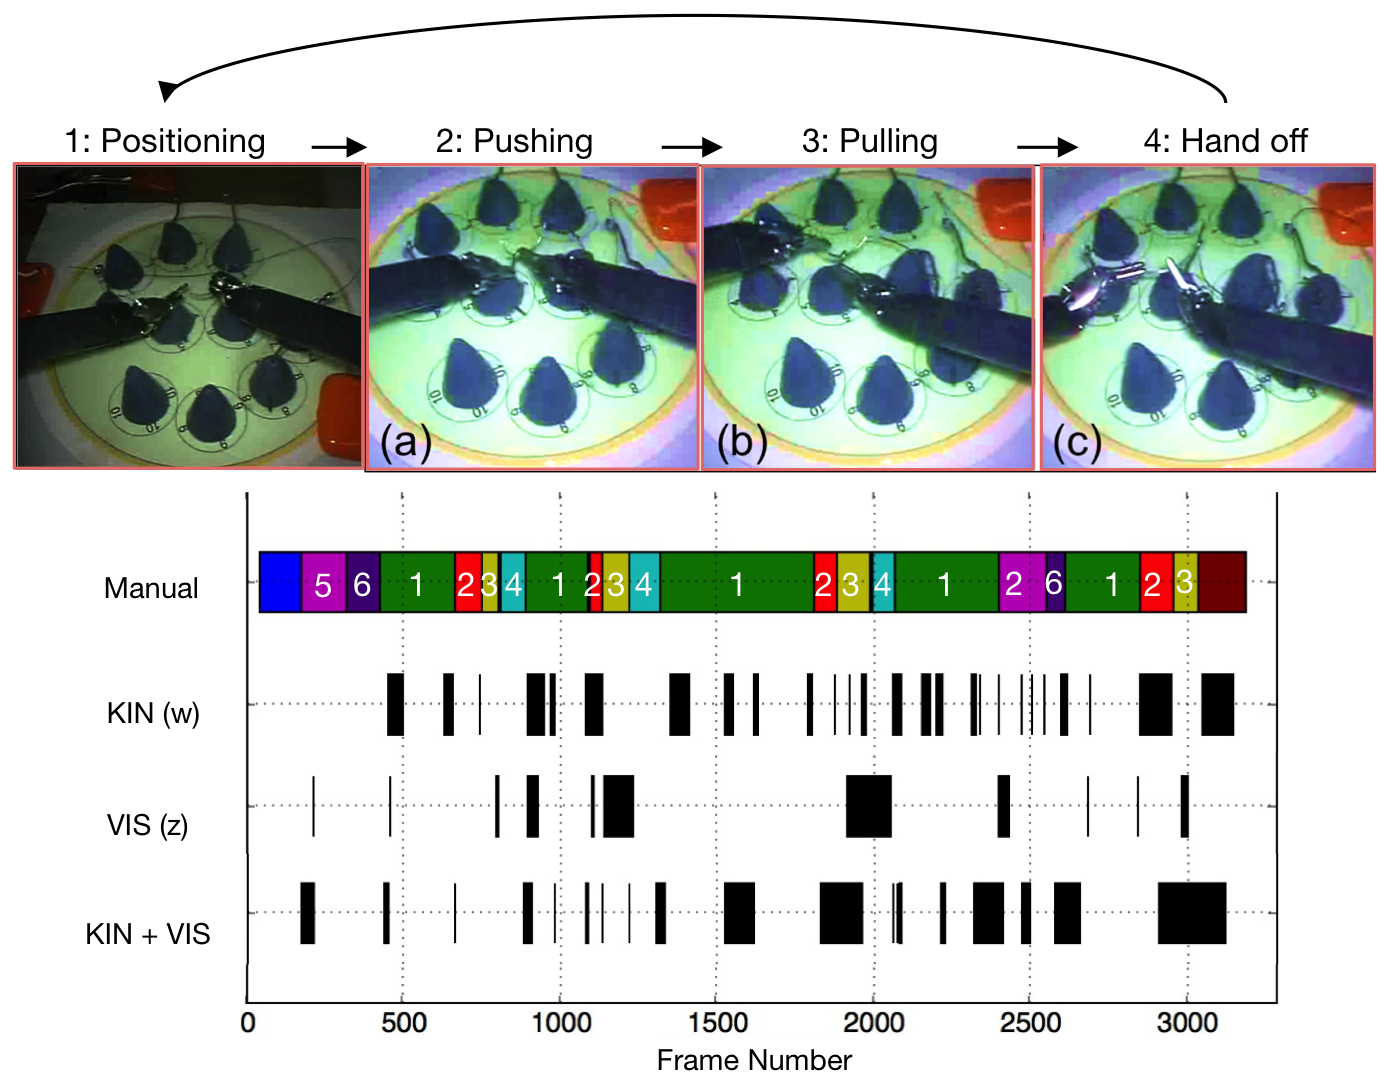
\includegraphics[width=\linewidth]{figures/needle_passing}
% 	\caption{Needle Passing}
% 	\label{fig:needlePassing}
% 	\vspace{-5pt}
% \end{figure}


% ==============================================

% \begin{algorithm}[t]
% \caption{The Transition State Clustering Algorithm \todo{Fix with changes} \label{algotext}}
% % \begin{algorithmic}[1]
% \scriptsize
% \State \textsf{Input: } $\mathcal{D}$, $\rho$ pruning parameter, and $\delta$ compaction parameter.

% \State $n(t) = \binom{\mathbf{x}(t+1)}{\mathbf{x}(t)}$. 

% \State Cluster the vectors $n(t)$ using DP-GMM assigning each state to its most likely cluster. 

% \State \emph{Transition states} are times when $n(t)$ is in a different cluster than $n(t+1)$. 

% \State Remove states that transition to and from clusters with less than a fraction of $p$ demonstrations. 

% \State Remove consecutive transition states when the L2 distance between these transitions is less than $\delta$. 

% \State Cluster the remaining transition states in the state space $\mathbf{x}(t+1)$ using DP-GMM.

% \State Within each state-space cluster, sub-cluster the transition states temporally. 

% \State \textsf{Output: } A set $\mathcal{M}$ of clusters of transition states and the associated with each cluster a time interval of transition times.
% % \end{algorithmic}
% \end{algorithm}

